\chapter{Twiz O' Meter in Ihrem Fahrzeug installieren}

Die Installation von ToM+ in Ihrem Twizy ist tatsächlich sehr einfach und erfordert keine besonderen
Kenntnisse, denn wie ich normalerweise sage, handelt es sich um ein „Plug-and-Drive“-Gerät! Befolgen Sie einfach diese wenigen
Schritte, um das Gerät schnell und korrekt zu installieren, oder wählen Sie selbst einen anderen Montageort.

\section{Position des LCD-Displays}

Bei der Bestellung des Geräts können Sie den 3D-Standfuß zusätzlich zum Clip-on-Display auswählen.
Sie können das Display also auf zwei verschiedene Arten installieren: im Clip-on-Modus oder
mit dem 3D-Standfuß. Der Clip-on-Modus ist am häufigsten und ermöglicht es Ihnen, das
Display am Dashboard des Fahrzeugs zu befestigen, während Sie das Display mit dem 3D-Standfuß
auf einer ebenen Fläche im Fahrzeug platzieren können (ich empfehle normalerweise das rechte oder linke Handschuhfach).

\subsection{Clip-on-Modus}

Wenn Sie diesen Modus wählen, ist die Installation wirklich einfach. Sie müssen das Display lediglich am
Dashboard befestigen, an einer Position, die für Sie während der Fahrt gut sichtbar und bequem ist. Setzen Sie den oberen
Teil des Displays auf das Dashboard und drücken Sie anschließend den unteren Teil nach unten, bis er einrastet.

\begin{figure}[H]
    \centering
    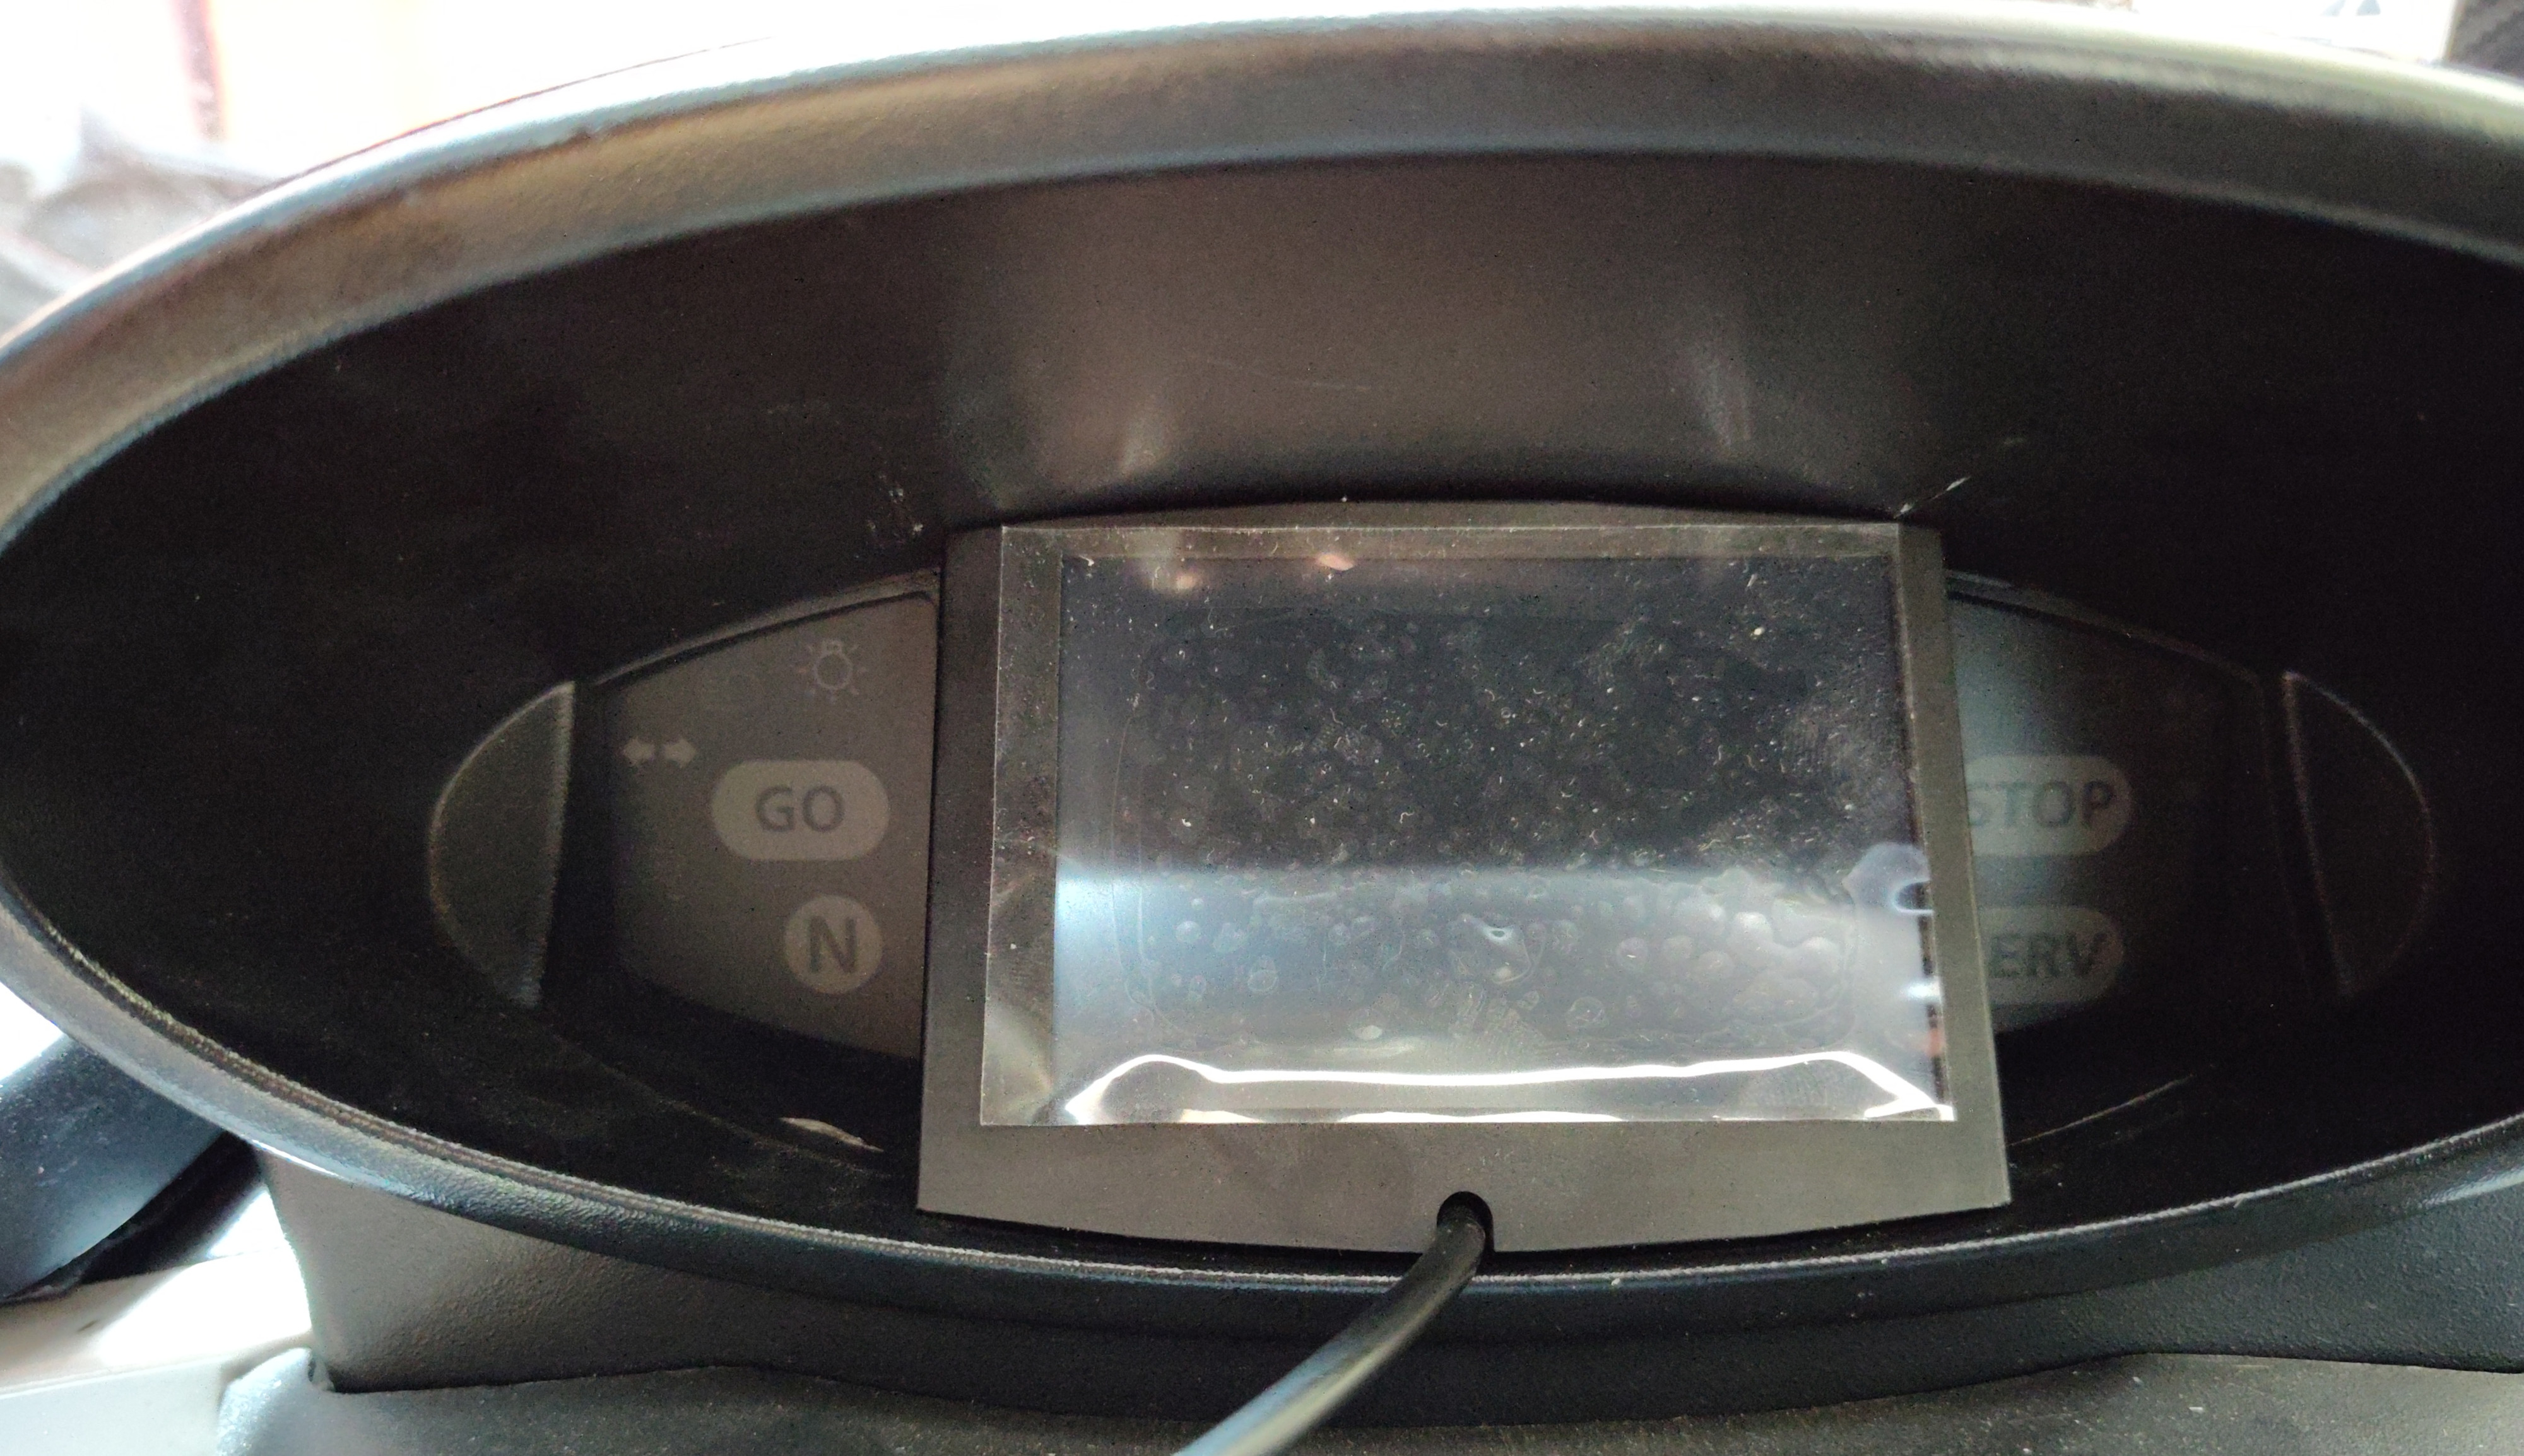
\includegraphics[width=0.8\textwidth]{figures/clip_on.jpg}
    \caption{Installation im Clip-on-Modus}
\end{figure}

Achten Sie darauf, dass das Kabel nicht im unteren Teil des Displays eingeklemmt wird, sondern sich frei
durch die dafür vorgesehene Öffnung bewegen kann. Andernfalls könnte das Kabel beschädigt werden.

\subsection{3D-Standfuß-Modus}

Falls mitgeliefert, können Sie den 3D-Standfuß verwenden, um das Display auf einer ebenen Fläche im Fahrzeug zu platzieren.
Sie können doppelseitiges Klebeband an der Unterseite anbringen, um ihn auf der Oberfläche zu befestigen.
Alternativ können Sie die Schraublöcher an der Unterseite des Standfußes verwenden, um ihn mit zwei Schrauben zu befestigen.

Wie beim Clip-on-Modus sollten Sie darauf achten, dass das Kabel beim Anbringen der Abdeckung nicht im hinteren Teil des Displays eingeklemmt wird,
sondern sich frei durch die dafür vorgesehene Öffnung bewegen kann. Andernfalls könnte das Kabel beschädigt werden.
Siehe Abbildung~\ref{fig:back_cover} und Abbildung~\ref{fig:bottom_cover_screwholes} auf Seite~\pageref{fig:back_cover}, um die genannten Teile zu sehen.
So sieht der 3D-Standfuß ohne installiertes Display aus.

\begin{figure}[H]
    \centering
    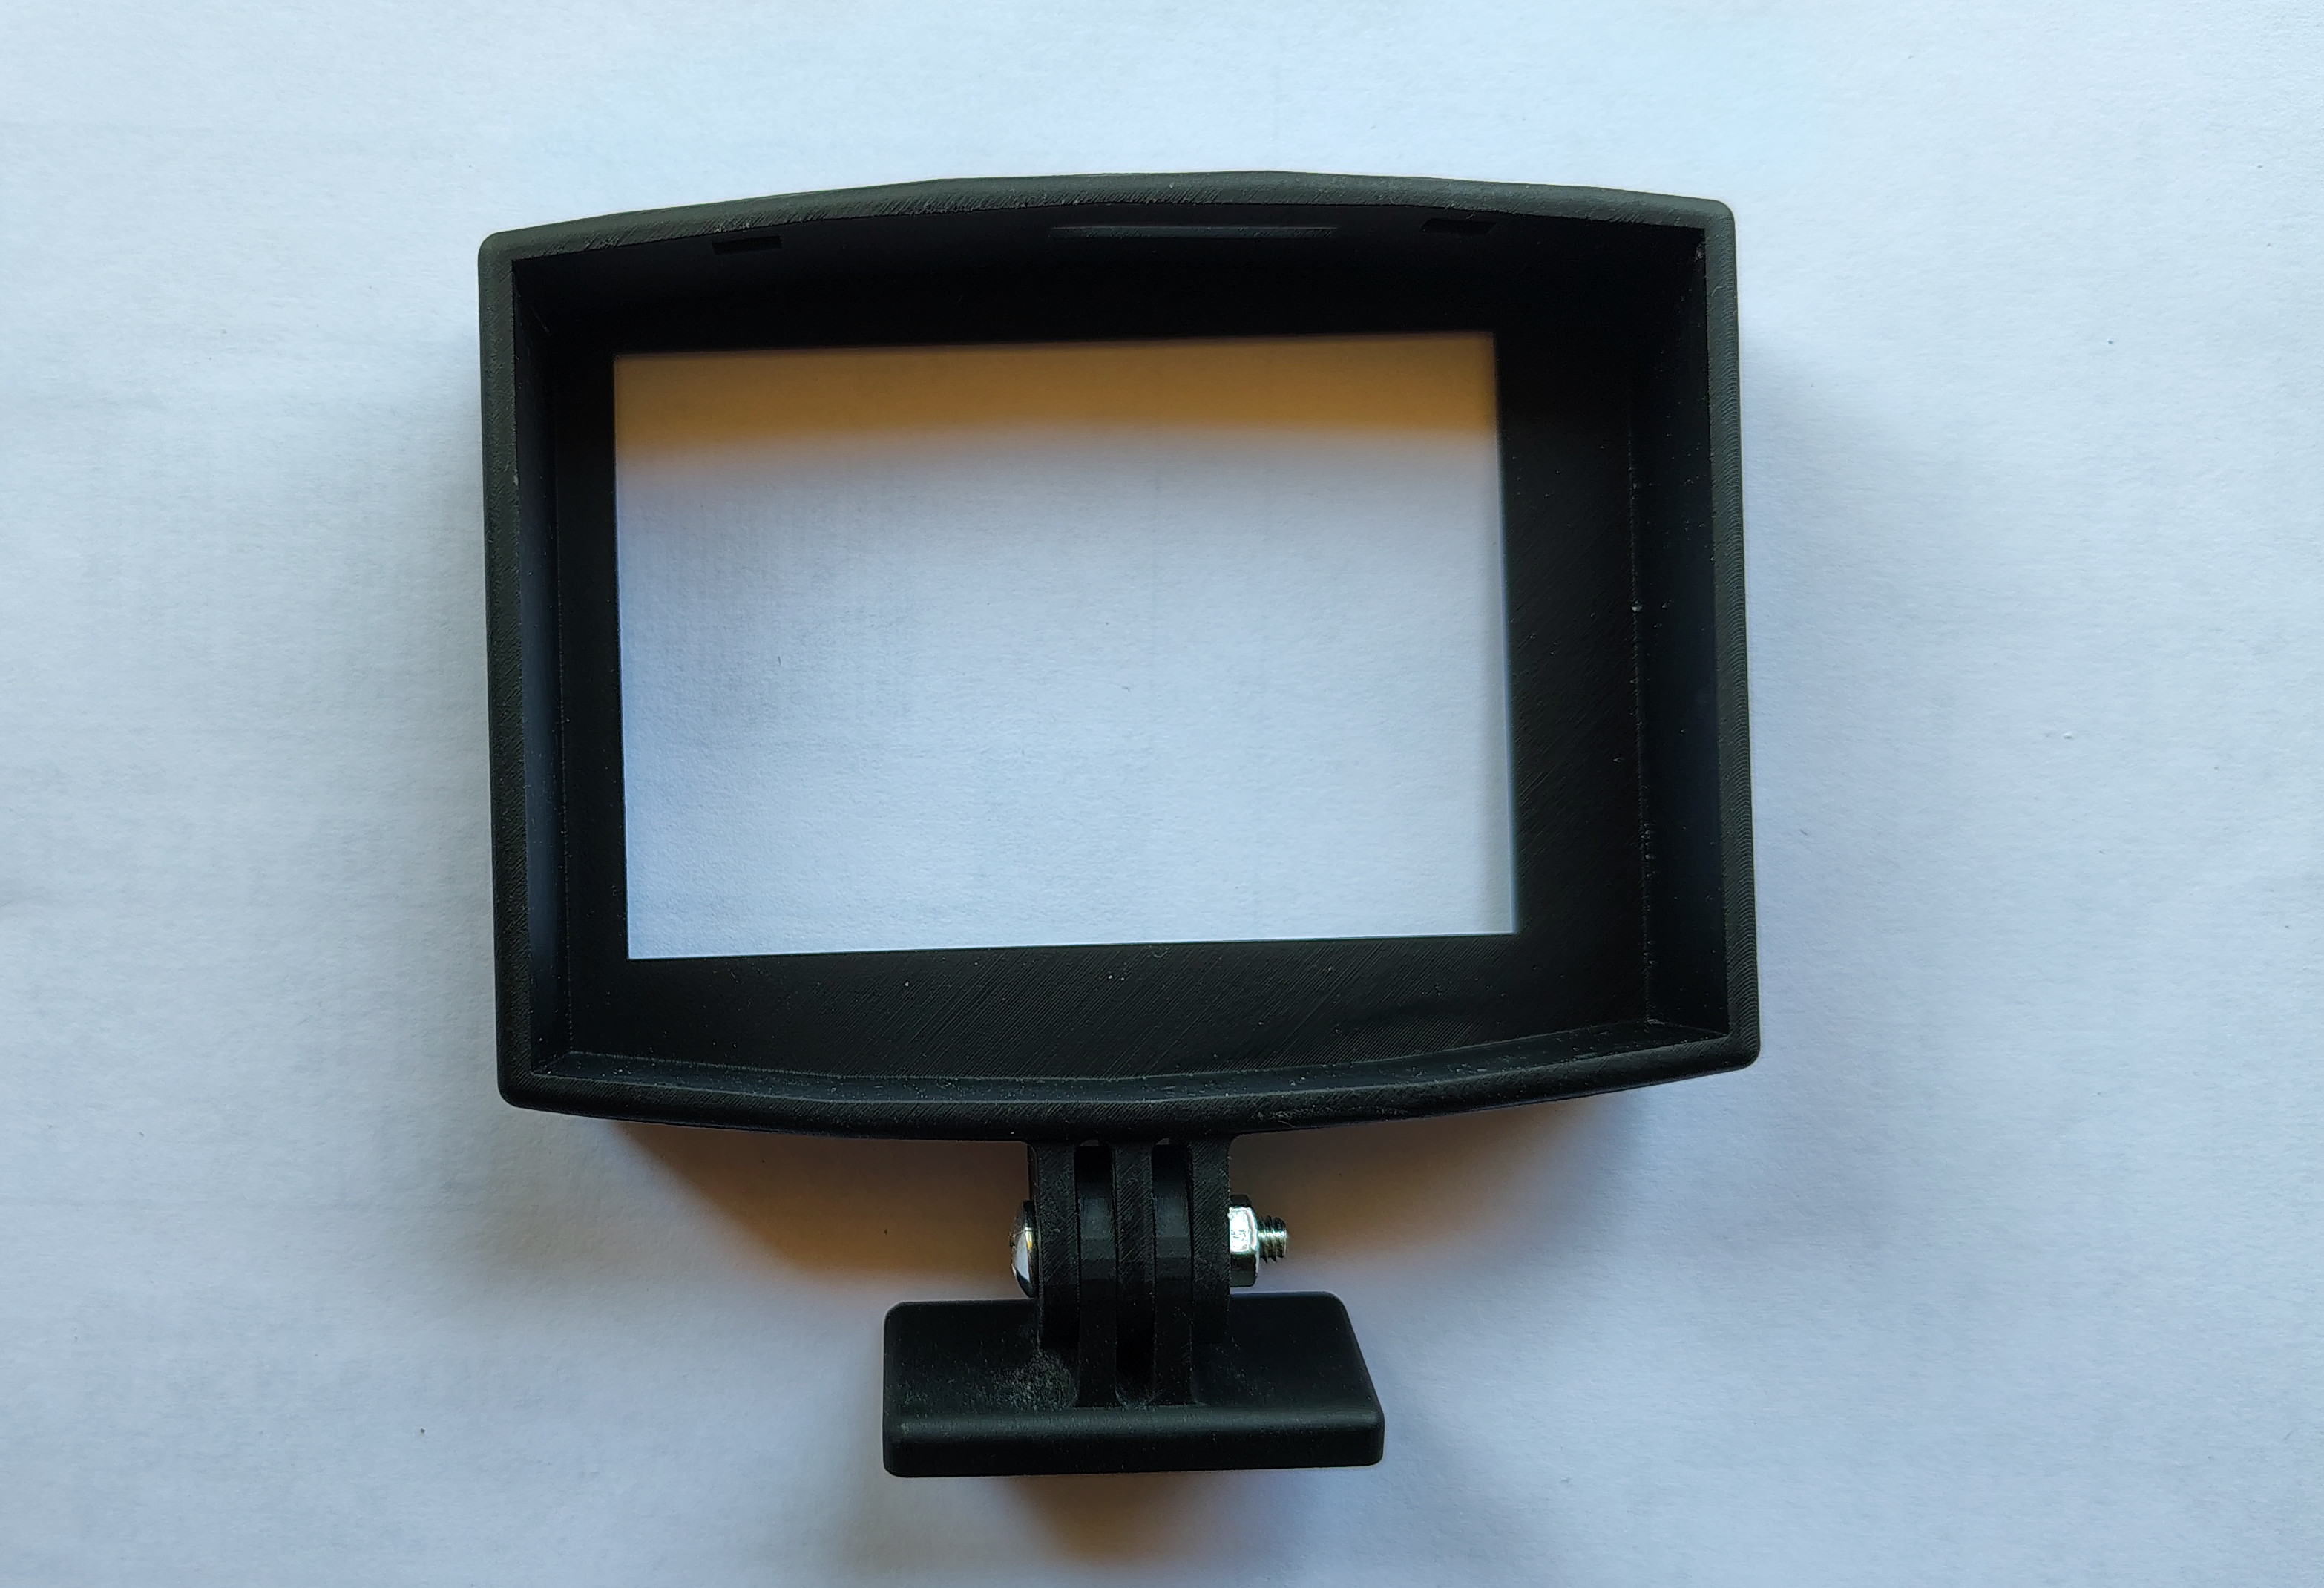
\includegraphics[width=0.8\textwidth]{figures/3d_stand.jpg}
    \caption{Leerer 3D-gedruckter Standfuß}
\end{figure}

\subsection{Kabelanschluss}

Anschließend können Sie die Schutzfolie vom Display entfernen und das Kabel anschließen, um es mit Strom zu versorgen.
Das andere Ende des Kabels muss mit der Black Box verbunden werden, die im nächsten Schritt installiert wird.
Der Stecker passt nur in einer Richtung. Achten Sie daher darauf, den Anschluss korrekt auszurichten, bevor Sie ihn einstecken.

\begin{figure}[H]
    \centering
    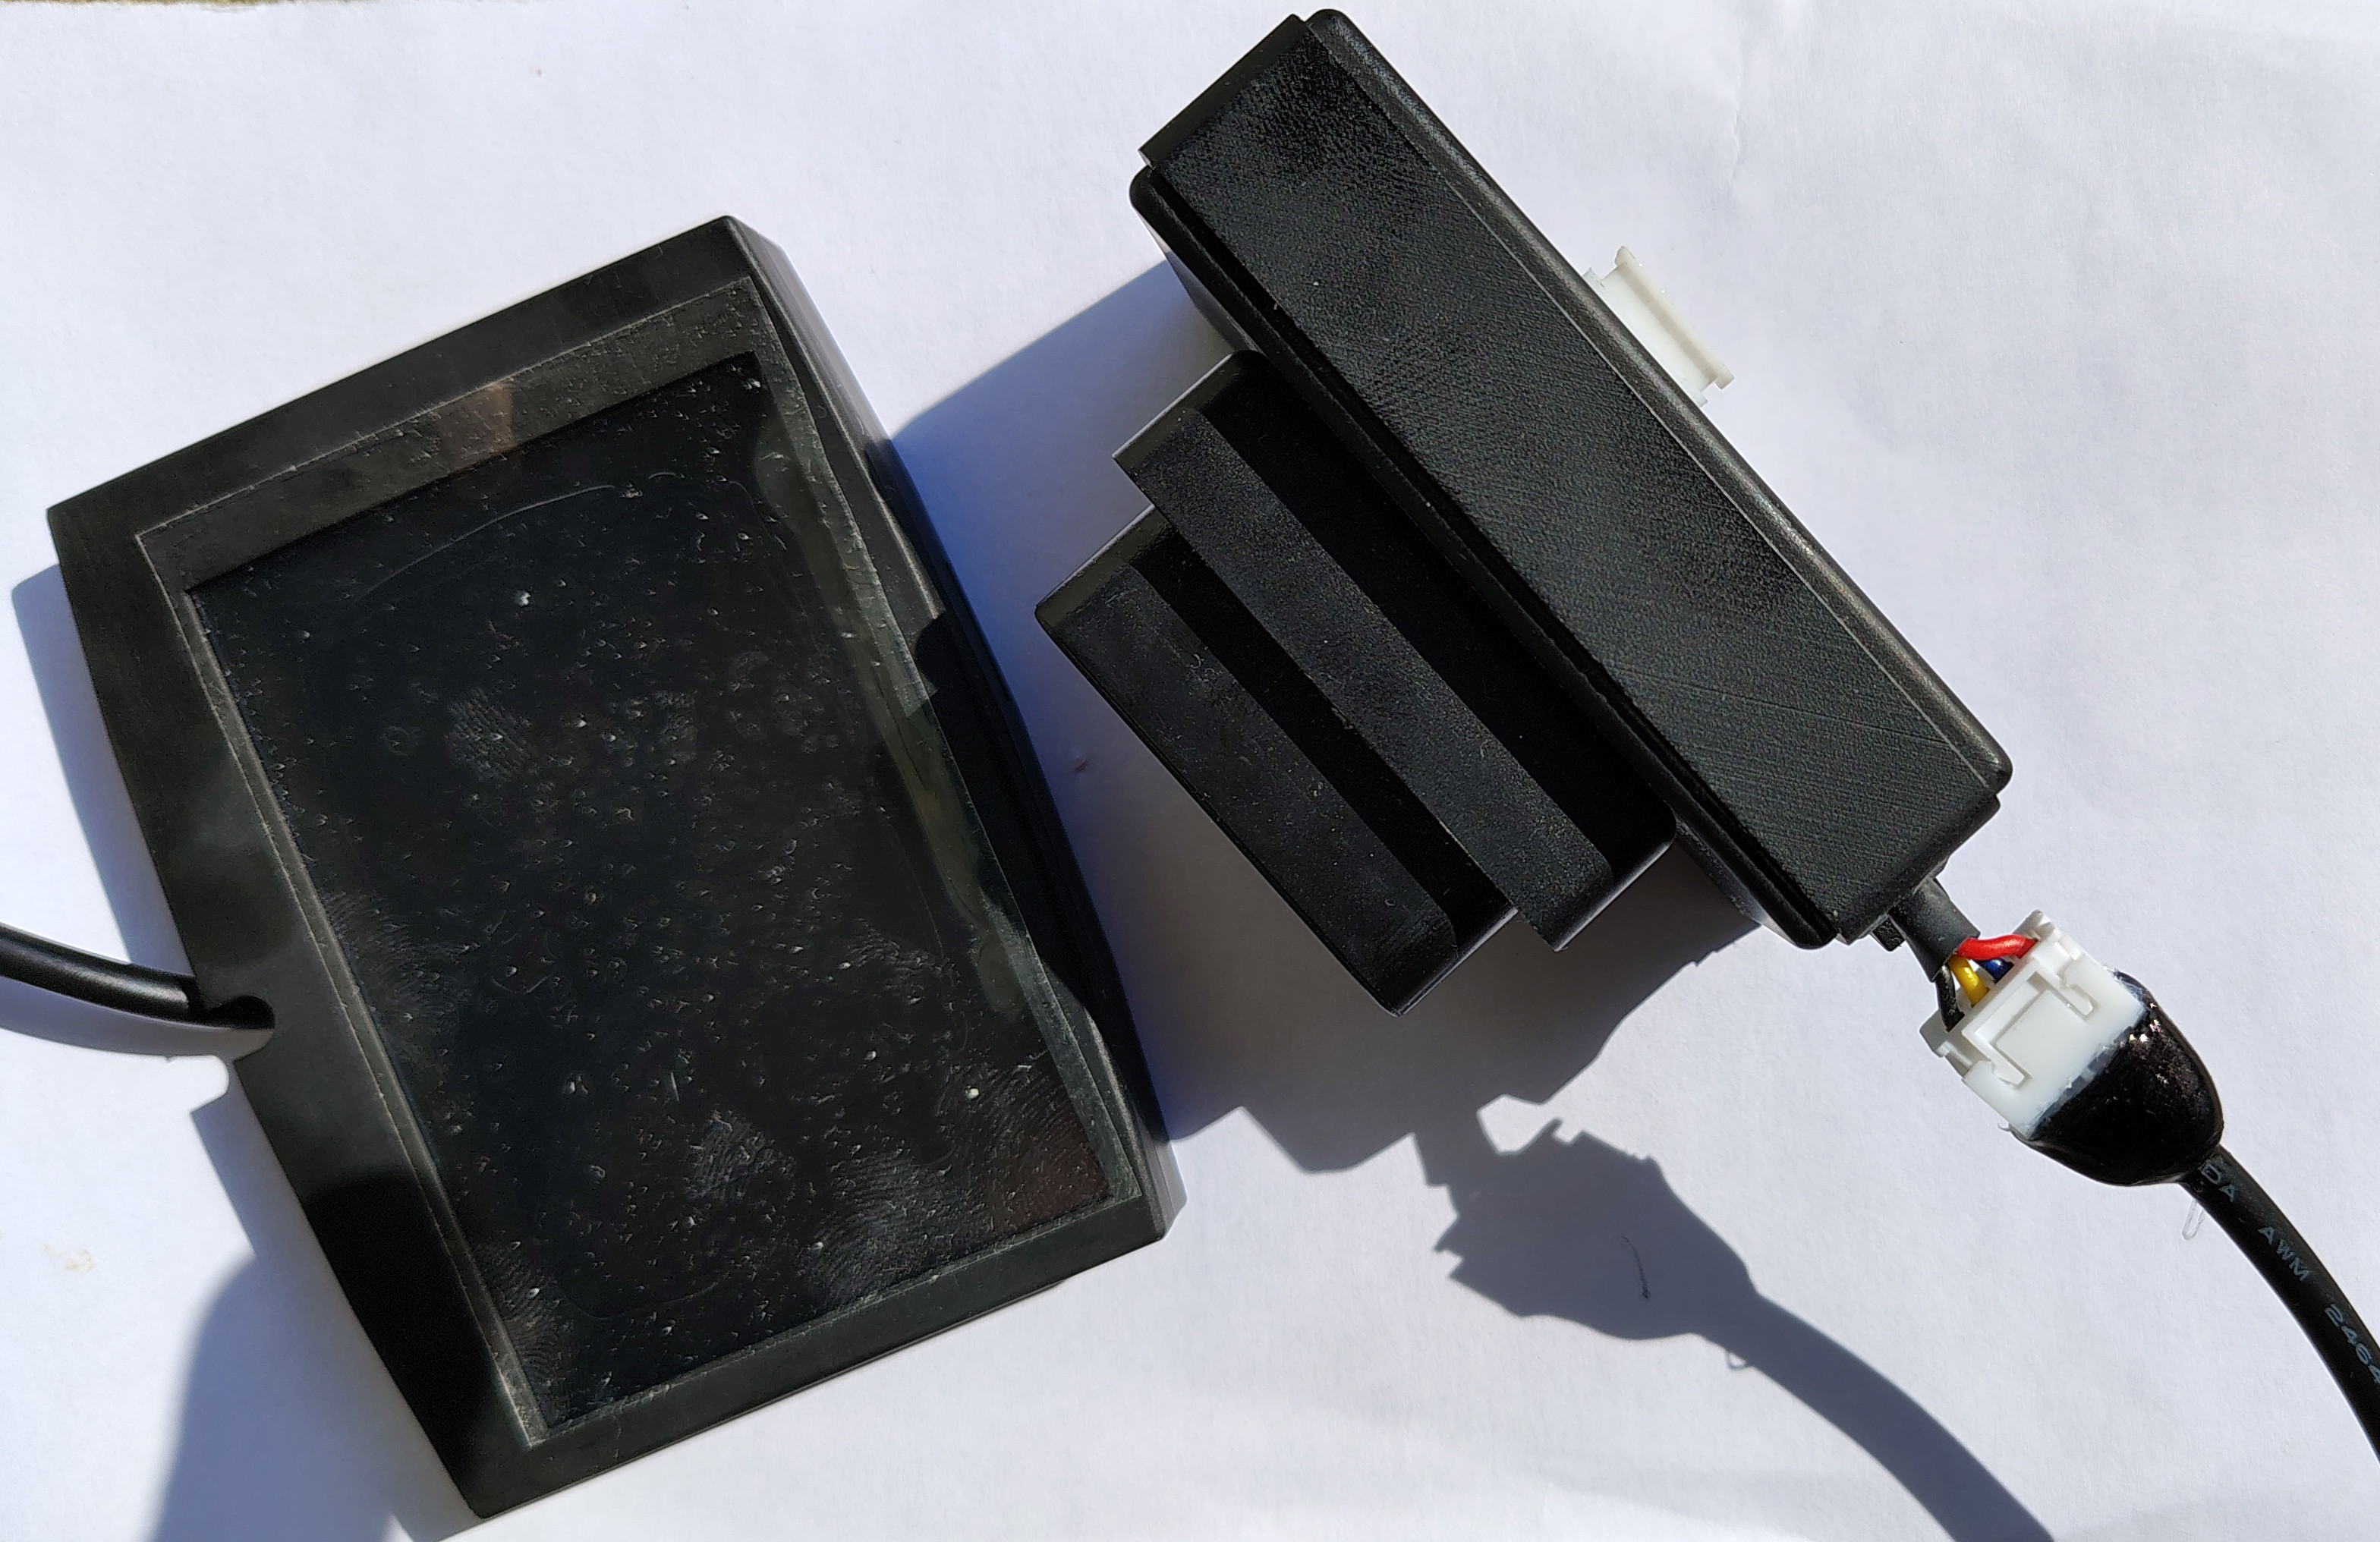
\includegraphics[width=0.8\textwidth]{figures/bb_connection.jpg}
    \caption{Anschluss der Black Box}
\end{figure}

\section{Position der Black Box}

Nachdem Sie entschieden haben, wo das Display platziert werden soll, müssen Sie die Black Box anschließen.

Die Black Box muss mit dem OBD2-Anschluss des Fahrzeugs verbunden werden, der sich im
linken Handschuhfach des Twizy befindet. Wenn Sie es noch nie geöffnet haben, finden Sie dort eine kleine Kunststoffabdeckung,
die Sie entfernen müssen, um Zugang zum OBD2-Anschluss zu erhalten. Sobald Sie Zugang haben, stecken Sie die
Black Box einfach ein und stellen Sie sicher, dass sie sicher verbunden ist. Der Stecker passt nur in eine Richtung. Achten Sie daher darauf,
den Anschluss korrekt auszurichten, bevor Sie ihn einstecken.

\begin{figure}[H]
    \centering
    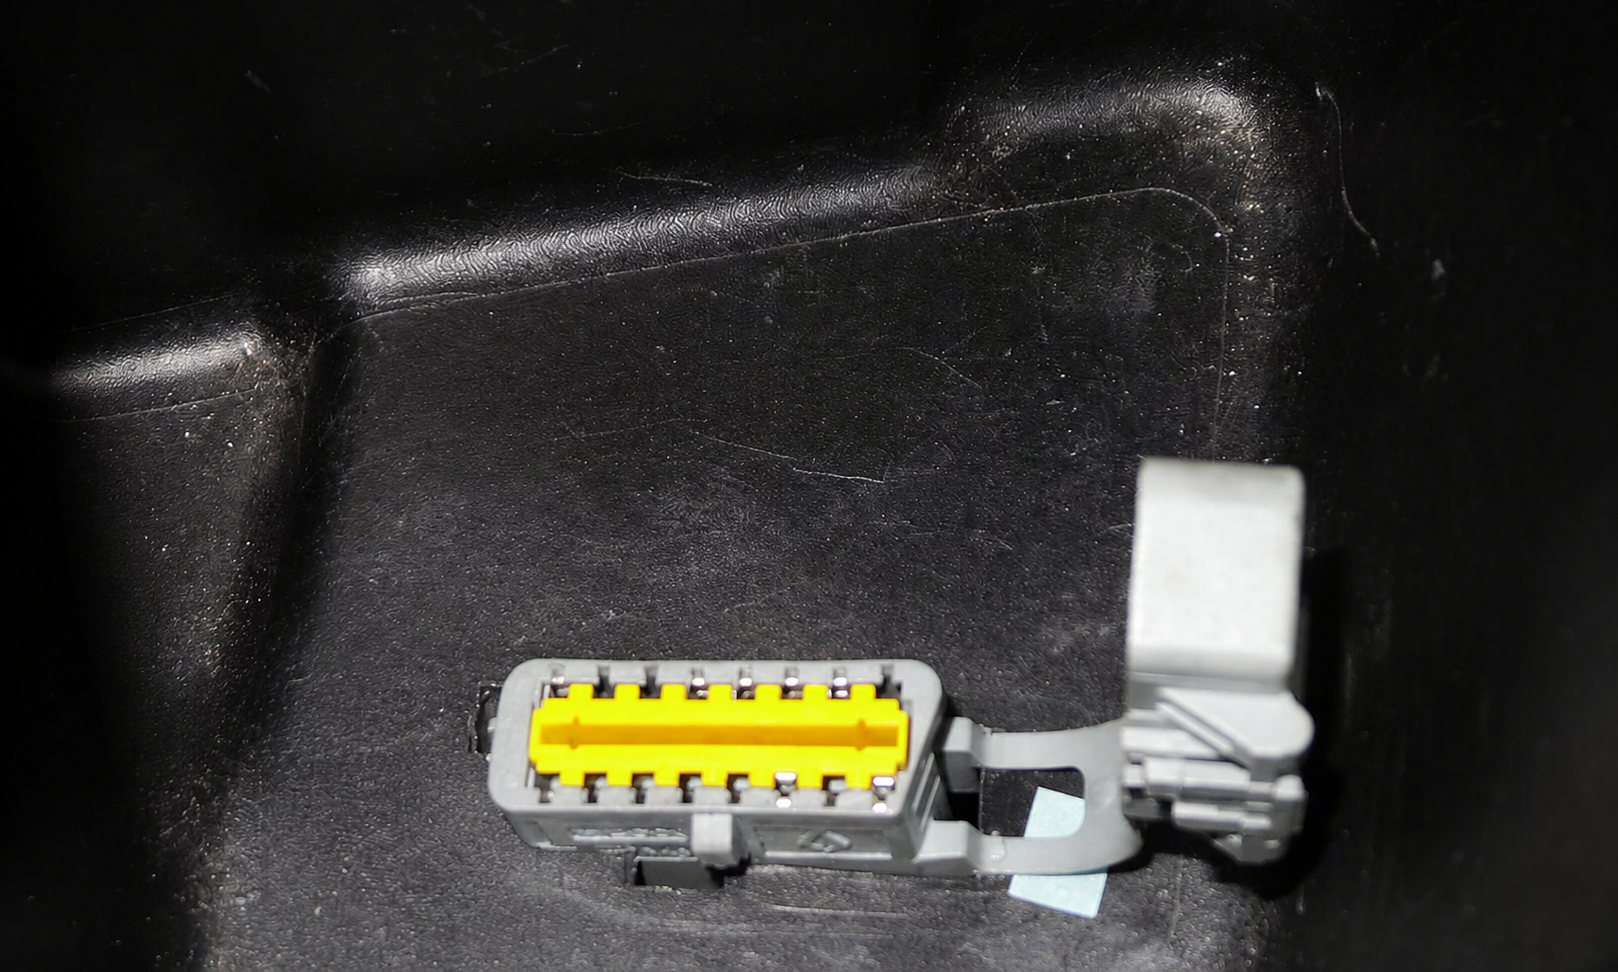
\includegraphics[width=0.8\textwidth]{figures/obd_connector.png}
    \caption{Position des OBD2-Anschlusses im Twizy}
\end{figure}

\textbf{Erst nachdem das Display angeschlossen wurde}, können Sie den Schalter an der Black Box einschalten.
Damit ist die Installation abgeschlossen! Jetzt können Sie Ihren Twizy starten und die ToM+-Funktionen genießen.
